\section{Context-Free Grammar Definition}
A CF grammar is described by $T$, $NT$, $S$, $PR$:
\begin{description}
    \item[$T$:] terminals/tokens of the language;
    \item[$NT$:] non-terminals (sets of strings generated by the grammar;
    \item[$S$:] start symbol ($S \in NT$);
    \item[$PR$:] production roles (indicate how $T$ and $NT$ are combined to generate valid strings).
\end{description}

Derivation is a sequence of grammar rule applications and substitutions (production rules) that transform a starting non-terminal into a sequence of terminals (tokens).
Example:
\begin{lstlisting}
assign_stmt ::= ID EQ exprs S;
expr ::= expr operator term;
term ::= ID;
term ::= INT;
...
\end{lstlisting}

\section{How Bottom-Up Parsing Works: Shift/Reduce Technique}
A stack, initially empty, is used to keep track of symbols already recognized.
Terminal symbols are pushed in the stack (shift), until the top of the stack contains a handle (right hand side of a production): the handle is then substituted by the corresponding non-terminal (reduce).
Note that the reduce operation may only be applied to the top of the stack.

Parsing is successful only when at the end of the input stream the stack contains only the start symbol.
Example:
\begin{itemize}
    \item[] input string: ``$a_1, a_2, a_3$''
    \item[] recursive left grammar:
    \begin{lstlisting}
list ::= list CM EL
list ::= EL
    \end{lstlisting}
    \item[] scanner: ``$a_1, a_2, a_3$'' $\Rightarrow$ \code{EL CM EL CM EL}
    \item[] parse tree:
    \begin{figure}[H]
        \centerline{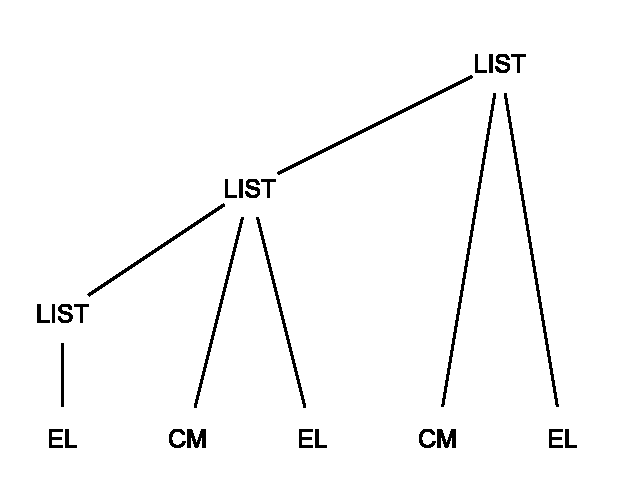
\includegraphics[width=0.5\textwidth]{img/17.pdf}}
    \end{figure}
    \item[] actions:
    \begin{table}[h]
        \centering
        \begin{tabular}{l|l}
            Action & Stack \\ \hline
             & $\varepsilon$ \\ \hline
            shift & \code{EL} \\ \hline
            reduce & \code{LIST} \\ \hline
            shift & \code{LIST CM} \\ \hline
            shift & \code{LIST CM EL} \\ \hline
            reduce & \code{LIST} \\ \hline
            shift & \code{LIST CM} \\ \hline
            shift & \code{LIST CM EL} \\ \hline
            reduce & \code{LIST} \\ \hline
        \end{tabular}
    \end{table}
\end{itemize}

\section{Introduction to CUP}
CUP is a parser generator that transforms the definition of a context-free grammar in a Java program that parses sequences of input symbols according to the grammar itself.
Besides defining syntax rules, it is possible to specify actions to be executed whenever a production is reduced.
The parser must be integrated by a scanner: some conventions simplify the integration of CUP-generated parses with JFlex-generated scanners.

\subsection{Source File Format}
A CUP source file has a syntax that is very similar to a Java program's one.
It can be ideally divided in the following sections:
\begin{enumerate}
    \item
    setup;
    \item
    terminals and non-terminals;
    \item
    precedences;
    \item
    rules.
\end{enumerate}

Comments are allowed to follow Java syntax.

\subsection{Setup Section}
This section contains all the directives needed for the parser, such as inclusion of CUP library and other libraries (\code{import java_cup.runtime.*;}).
In this section there is also a user code part, in which there are redefinitions of cup internal methods and integration with another scanner other than JFlex.

\subsection{Terminals/Non-Terminals Section}
It contains the definition of:
\begin{itemize}
    \item
    the grammar start symbol;
    \item
    terminals (passed by JFlex);
    \item
    non-terminals.
\end{itemize}

More specifically:
\begin{description}
    \item[start symbol]
    \begin{itemize}
        \item
        ``start with \code{<non_terminal_name>}'',
        \item
        it is the root of the parse tree,
        \item
        only one occurrence of this keyword is allowed;
    \end{itemize}
    \item[terminals]
    \begin{itemize}
        \item
        ``terminal \code{<term_1>}, \code{<term_2>}, \ldots'',
        \item
        \code{<term>} name contains letters, ``\_'', ``.'', and digits (the first character must be a letter),
        \item
        terminals are recognized by JFlex;
    \end{itemize}
    \item[non-terminals]
    \begin{itemize}
        \item
        ``non-terminal \code{<n_term_1>}, \code{<n_term_2>}'',
        \item
        \code{<n_term>} name contains letters, ``\_'', ``.'', and digits (the first character must be a letter).
    \end{itemize}
\end{description}

Example:
\begin{figure}[H]
    \centerline{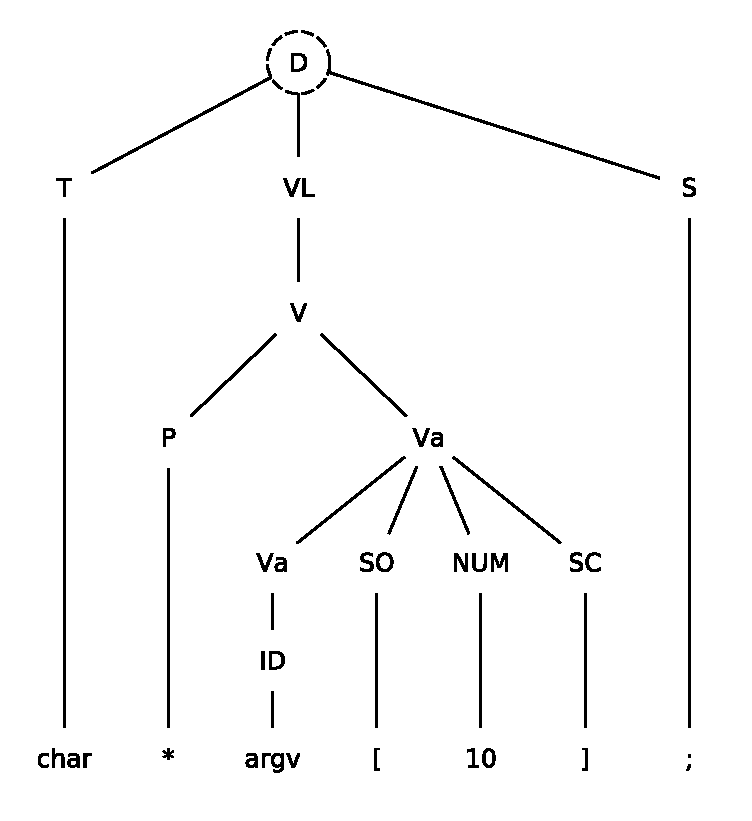
\includegraphics[width=0.5\textwidth]{img/18.pdf}}
\end{figure}
Productions (grammar rules):
\begin{align*}
    D &\to T \quad VL \quad S \\
    VL &\to V \\
    VL &\to VL \quad CM \quad V \\
    V &\to P \quad V \\
    V &\to Va \\
    Va &\to Va \quad SO \quad NUM \quad SC \\
    Va &\to ID
\end{align*}
Input string: \code{char * argv[10]}

\subsection{Rules Section}
The rules section contains one or more productions in the form of:
\begin{lstlisting}
<non_terminal> ::= right_hand_side;
\end{lstlisting}
Where \code{right_hand_side} is a sequence of zero or more symbols.

To each production, an action can be associated, which must be enclosed between ``\code{\{:}'' and ``\code{:\}}''.
Note that the action is executed right before the reduce action takes place.

Example:
\begin{lstlisting}
D ::= T VL S {:
        System.out.println("Declaration found.");
    :}
;
\end{lstlisting}

If more than one production exist for a given non-terminal, they must be grouped and separated by ``\code{\|}''.

Example:
\begin{lstlisting}
funz ::= type ID RO VL RC S {:
        System.out.println("Function prototype");
    :}
    | ::= type ID RO VL RC BO stmt_list BC {:
        System.out.println("Function");
    :}
;
\end{lstlisting}
Note that the use of the ``\code{\|}'' character generates two separated rules.
It is important to remember that the code between ``\code{\{:}'' and ``\code{:\}}'' is executed only when a given rule is matched.

Example:
\begin{lstlisting}[frame=single]
// terminals - non-terminals section
terminal T, P, ID, NUM, S, CM, SO, SC;
non terminal D, V, VL, Va;
start with D;

// rules section
D ::= T VL S;
VL ::= V | VL CM V;
V ::= P V | Va
Va ::= Va SO NUM SC | Va
\end{lstlisting}
Productions:
\begin{align*}
    D &\to T \quad VL \quad S \\
    VL &\to V \\
    VL &\to VL \quad CM \quad V \\
    V &\to P \quad V \\
    V &\to Va \\
    Va &\to Va \quad SO \quad NUM \quad SC \\
    Va &\to ID
\end{align*}

\section{Integrating JFlex and CUP}
\begin{figure}[H]
    \centerline{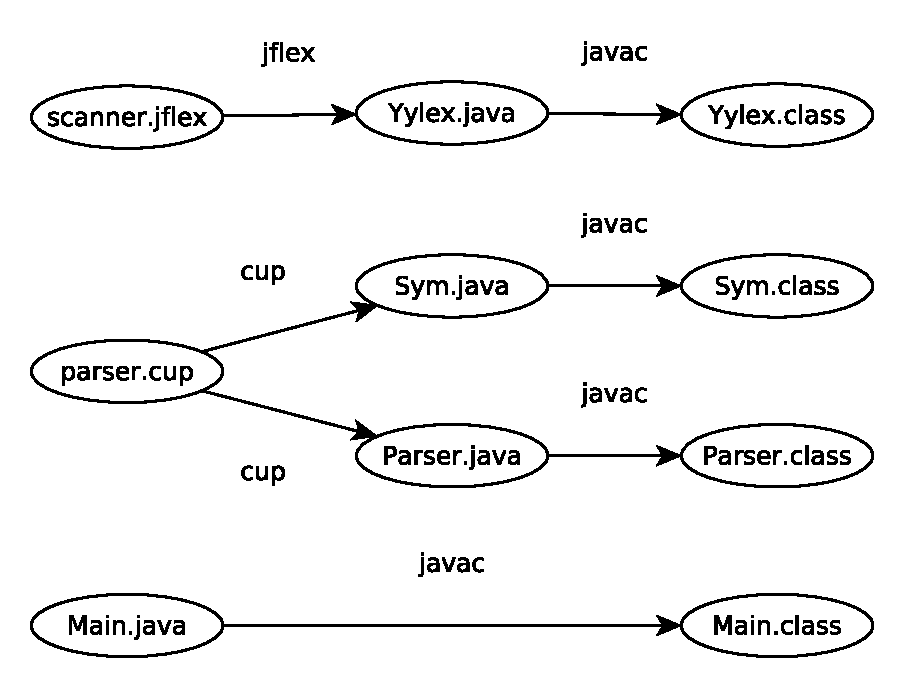
\includegraphics[width=0.6\textwidth]{img/19.pdf}}
\end{figure}

Parser and scanner must agree on the values associated to each token (terminal).
When the scanner recognizes a token, it must pass a suitable value to the parser.
This is done by means of the \emph{Symbol} class, whose constructors are:
\begin{itemize}
    \item
    \code{public Symbol (int sym_id)};
    \item
    \code{public Symbol (int sym_id, int left, int right)};
    \item
    \code{public Symbol (int sym_id, Object O)};
    \item
    \code{public Symbol (int sym_id, int left, int right, Object O)}.
\end{itemize}
The class \emph{Symbol} can be found in the CUP installation directory \code{java_cup/runtime/Symbol.java}.

When a terminal is defined by means of the terminal keyword, cup associates an integer value to that token.
This mapping is contained in the \code{Sym.java} generated by CUP during compiling processes.

Example: if in the parser the following list of terminal symbols has been declared
\begin{lstlisting}
terminal T, P, ID, NUM, PV, CM, SO, SC, S;
\end{lstlisting}
they can be used inside the scanner and passed to the parser in the following way:
\begin{lstlisting}[frame=single]
...
%%
...
%%
[a-zA-Z_][a-zA-Z0-9_]* {return new Symbol(sym.id);}
\[ {return new Symbol(sym.SO);}
\] {return new Symbol(sym.SC);}
\end{lstlisting}

\subsection{Scanner Modifications}
It includes the CUP library (\code{java.cup.runtime.*}) in the code section; it also activates CUP compatibility by means of the \code{\% cup} directive in the declaration section.

Example:
\begin{lstlisting}[frame=single]
...
%%
% cup
...
%%
[a-z]+ {return new Symbol(sym.EL);}
"," {return new Symbol(sym.CM);}
\end{lstlisting}

\subsection{The CUP Parser}
Example:
\begin{lstlisting}[frame=single]
import java_cup.runtime.*;

terminal EL, CM;
non terminal LIST, ELIST;
start with ELIST;

ELIST ::= LIST {:
        System.out.println("list found");
    :}
    | {:
        System.out.println("empty list");
    :}
;

LIST ::= LIST CM EL
;

LIST ::= EL
;
\end{lstlisting}

\subsection{Main File (\code{Main.java})}
Example:
\begin{lstlisting}[frame=single]
import java.io.*;

public class Main {
    static public void main(String argv[]) {
        try {
            // instantiate the scanner and open input file argv[0]
            Yylex L = new Yylex(new FileReader(argv[0]));
            // instantiate the parser
            Parser p = new Parser(L);
            // start the parser
            Object result = p.parse();
        } catch(Exception e) {
            e.printStackTrace();
        }
    }
}
\end{lstlisting}

\subsection{Compiling Steps}
\begin{enumerate}
    \item
    \code{jflex scanner.jflex}
    \item
    \code{java java_cup.Main parser.cup}\footnote{Note that in case of shift/reduce or reduce/reduce conflicts, the command is: \code{java java_cup.Main -expect <#conflicts> parser.cup}}
    \item
    \code{java java_cup.MainDrawTree parser.cup}\footnote{\code{MainDrawTree} is for debugging purpose.}
    \item
    \code{javac Yylex.java Sym.java Parser.java Main.java} or \code{javac *.java}\footnote{This is to compile all the files of the project.}
    \item
    \code{java Main <file>}\footnote{This is to execute the program using \code{<file>} as input.}
\end{enumerate}